
% Slide 1: three Table 1 presets, all replayed through both policies.
\begin{frame}[t]{Furuta: the three published HOLD attacks}
\small
\(\ell=25,\ \hat p_m=0.25,\ \bar a=4,\ \alpha=0.01,\ T_s=5\,\mathrm{ms}\).
The same schedule and initial state drive both policies.
\vspace{1mm}
\begin{columns}[T,onlytextwidth]
\column{0.51\textwidth}
\begin{tikzpicture}
\begin{axis}[trace,width=\linewidth,height=3.65cm,
 xlabel={Time after initial forced hit (s)},ylabel={Pendulum angle (deg)},
 xmin=0,xmax=.125,ymin=-24,ymax=4,
 legend style={at={(.02,.03)},anchor=south west,font=\tiny,draw=none,fill=white},
 legend columns=2]
\addplot[holdred,thick,] coordinates {(0,0.5731552492) (0.005,0.562169538) (0.01,0.4985888844) (0.015,0.3820828321) (0.02,0.2120458485) (0.025,-0.01438817278) (0.03,-0.3003784578) (0.035,-0.6474114227) (0.04,-1.057290749) (0.045,-1.460833361) (0.05,-1.671777621) (0.055,-1.579928442) (0.06,-1.190562619) (0.065,-0.5016564478) (0.07,0.4903706165) (0.075,1.712267672) (0.08,2.676624247) (0.085,2.88379653) (0.09,2.245559595) (0.095,0.7585962475) (0.1,-1.584821909) (0.105,-4.643739351) (0.11,-8.280919318) (0.115,-12.51526582) (0.12,-17.36878659) (0.125,-21.75198247)};\addlegendentry{HOLD, \(n_w=10\)}
\addplot[blue,thick,] coordinates {(0,0.5731552492) (0.005,0.562169538) (0.01,0.4985888844) (0.015,0.3801004821) (0.02,0.2041061453) (0.025,-0.03030884528) (0.03,-0.3243628463) (0.035,-0.6795841844) (0.04,-1.066461047) (0.045,-1.328987201) (0.05,-1.32653314) (0.055,-1.043751086) (0.06,-0.4791712967) (0.065,0.3098699196) (0.07,1.26720288) (0.075,2.130908973) (0.08,2.478988649) (0.085,2.222320762) (0.09,1.428235349) (0.095,0.09260520089) (0.1,-1.791511533) (0.105,-4.233907427) (0.11,-7.070905883) (0.115,-10.14088122) (0.12,-13.45978945) (0.125,-16.02556158)};\addlegendentry{HOLD, \(n_w=12\)}
\addplot[orange,thick,] coordinates {(0,0.5731552492) (0.005,0.562169538) (0.01,0.4985888844) (0.015,0.3820828321) (0.02,0.2100634985) (0.025,-0.02034552597) (0.03,-0.3103417771) (0.035,-0.6614324918) (0.04,-1.075442441) (0.045,-1.504341655) (0.05,-1.760111189) (0.055,-1.69676499) (0.06,-1.30672478) (0.065,-0.5879633506) (0.07,0.3855656261) (0.075,1.223912398) (0.08,1.528060639) (0.085,1.213537782) (0.09,0.2787091129) (0.095,-1.281284079) (0.1,-3.474549757) (0.105,-6.215733162) (0.11,-9.422327299) (0.115,-13.11099824) (0.12,-16.24281245) (0.125,-16.99621636)};\addlegendentry{HOLD, \(n_w=14\)}
\addplot[zeroteal,thick,dashed] coordinates {(0,0.5731552492) (0.005,0.562169538) (0.01,0.5263472755) (0.015,0.4932606689) (0.02,0.4627377527) (0.025,0.4048791449) (0.03,0.3193841292) (0.035,0.2355490918) (0.04,0.1529383055) (0.045,0.05563556085) (0.05,-0.04759294443) (0.055,-0.1204862538) (0.06,-0.1726951481) (0.065,-0.2258016142) (0.07,-0.2800816697) (0.075,-0.3160593638) (0.08,-0.3160900955) (0.085,-0.2912470148) (0.09,-0.2592325941) (0.095,-0.2285655182) (0.1,-0.1990863967) (0.105,-0.1712592288) (0.11,-0.1449393847) (0.115,-0.1193728536) (0.12,-0.09442675529) (0.125,-0.07702961586)};
\addlegendentry{ZERO, \(n_w=10\)}
\end{axis}
\end{tikzpicture}
\column{0.46\textwidth}
\centering
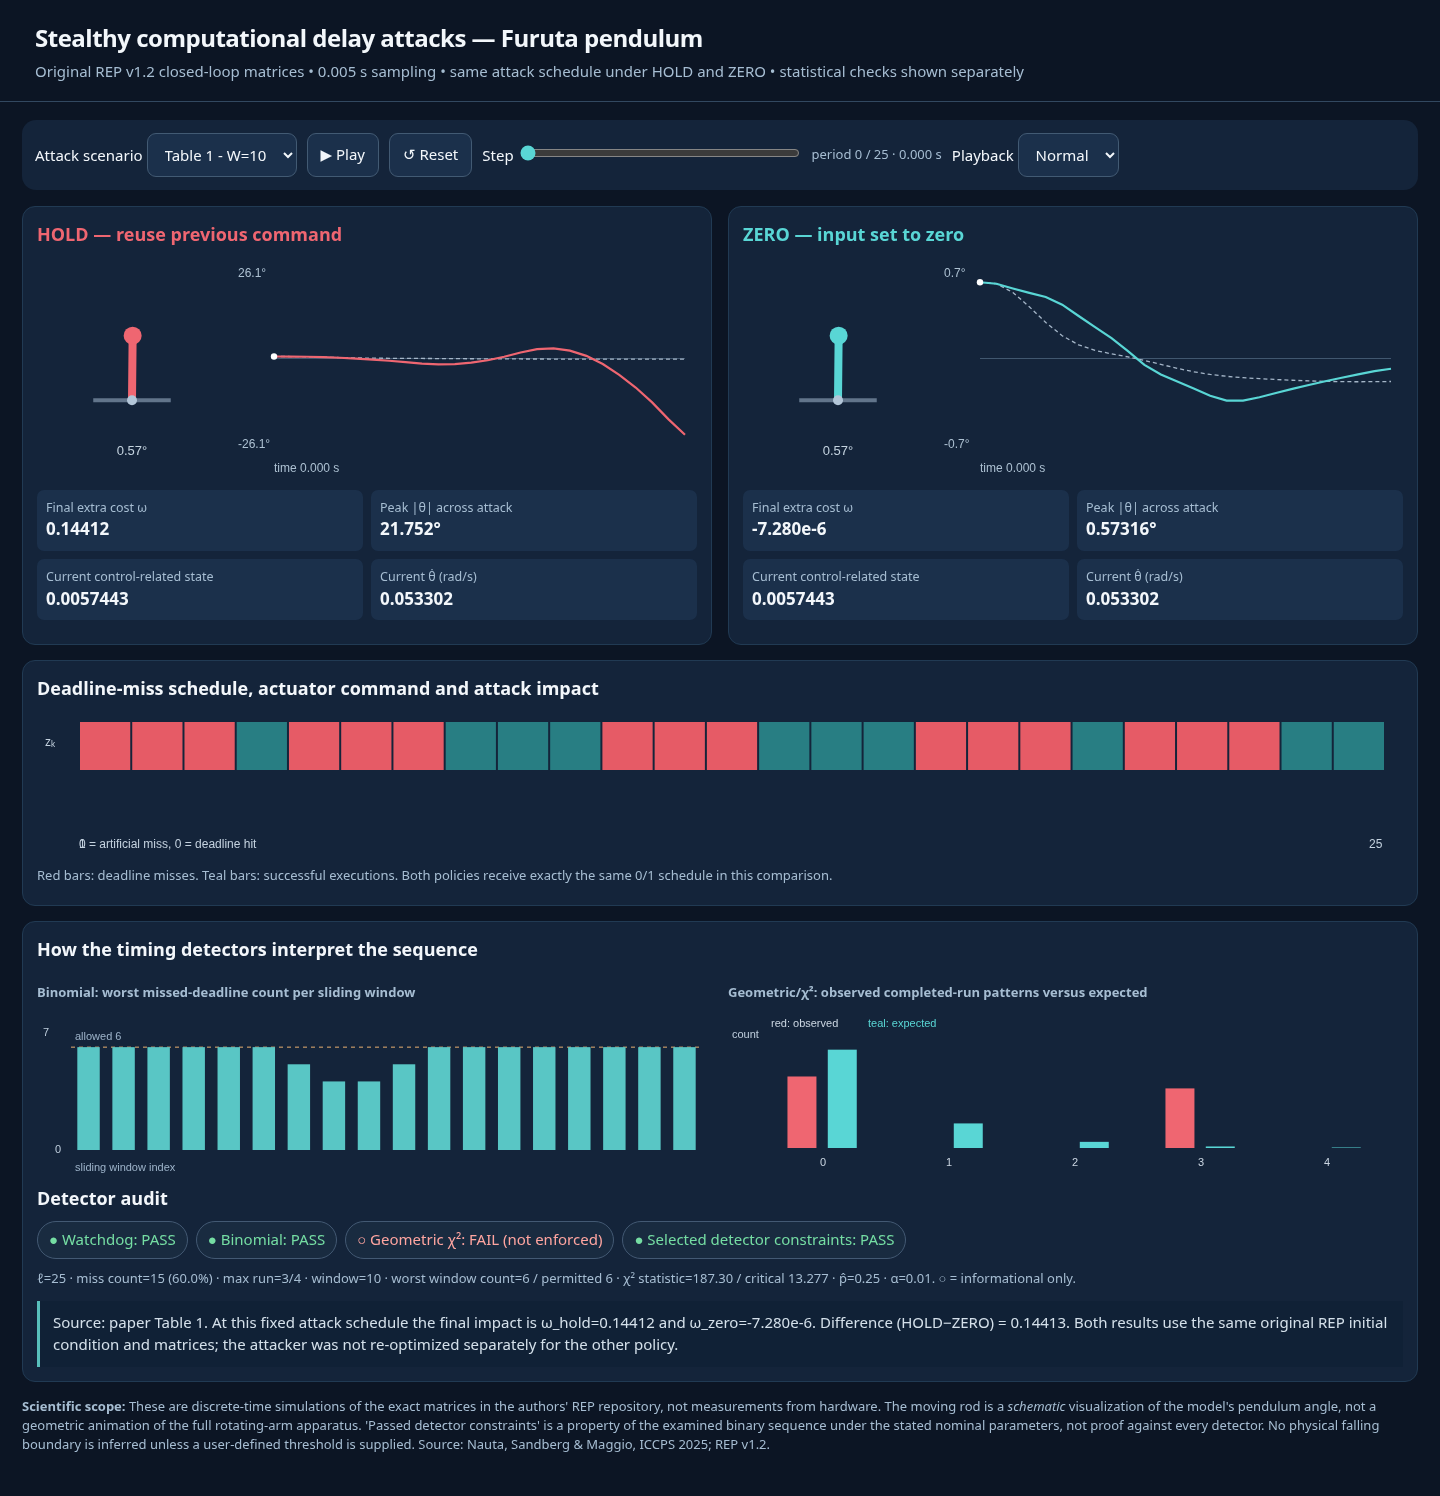
\includegraphics[trim=20bp 835bp 20bp 200bp,clip,width=\linewidth]{../../assets/srinjoy/furuta_dashboard.png}
\vspace{1mm}
\raggedright\footnotesize
Supplied dashboard: schematic angle view.
\par\vspace{2mm}
All pass watchdog and binomial. Geometric tests reject all three:
\(\chi^2=187.30,\ 86.22,\ 94.78>13.277\).
\end{columns}
\vspace{1mm}
\centering\footnotesize
\begin{tabular}{@{}ccrrr@{}}
\toprule
Window & Misses & \(\omega_{\rm HOLD}\) (rad\(^2\)) & \(\omega_{\rm ZERO}\), same attack & Peak \(|\theta|\), HOLD\\
\midrule
10 & 15 & 0.144120 & \(-7.28\!\times\!10^{-6}\) & 21.75$^\circ$ \\
12 & 14 & 0.078222 & \(-5.72\!\times\!10^{-6}\) & 16.03$^\circ$ \\
14 & 14 & 0.087986 & \(-7.36\!\times\!10^{-6}\) & 17.00$^\circ$ \\

\bottomrule
\end{tabular}
\par\vspace{1mm}\raggedright
\footnotesize\textbf{Validation:} same-schedule replay supports the paper's actuation-policy sensitivity.
\source{Paper Table 1 / Fig. 4; supplied ZIP: dashboard, Python replay and validated statistics.}
\note{All three published sequences and their detector audits come from the supplied ZIP.
The numerical routines in rep\_paper\_visuals.py were used unchanged. The zero-policy
curves use each HOLD-optimized sequence without re-optimizing. Negative omega means
that this fixed schedule has a smaller terminal angle cost than nominal at the scored
sample. It does not bound the ZERO worst case. Physical time starts after the first
forced hit. All values score the state before the last forced hit.
Source paper: https://doi.org/10.1145/3716550.3722013 .}
\end{frame}


% Slide 2: all remaining Furuta presets in the earlier reviewed visualization.
\begin{frame}[t]{Furuta: horizon and detector validation}
\small
The published ZERO cases use the combined detector with \(n_w=20\).
The earlier 23-period replay uses binomial detection with \(n_w=10\).
\vspace{2mm}
\begin{columns}[T,onlytextwidth]
\column{0.49\textwidth}
\begin{tikzpicture}
\begin{axis}[trace,width=\linewidth,height=4.45cm,
 xlabel={Time after initial forced hit (s)},ylabel={ZERO angle (deg)},
 xmin=0,xmax=.125,
 legend style={at={(.98,.98)},anchor=north east,font=\scriptsize,draw=none,fill=white}]
\addplot[blue,thick,] coordinates {(0,0.5731552492) (0.005,0.562169538) (0.01,0.5263472755) (0.015,0.4932606689) (0.02,0.4329970116) (0.025,0.3452430871)};\addlegendentry{\(\ell=5\)}
\addplot[holdred,thick,] coordinates {(0,0.5731552492) (0.005,0.562169538) (0.01,0.5263472755) (0.015,0.4635199278) (0.02,0.3733609538) (0.025,0.269948985) (0.03,0.1527465442) (0.035,0.03633799374) (0.04,-0.07504831727) (0.045,-0.1819913119) (0.05,-0.2898801947) (0.055,-0.399275711) (0.06,-0.486759363) (0.065,-0.5527858414) (0.07,-0.5828105344) (0.075,-0.5436788959)};\addlegendentry{\(\ell=15\)}
\addplot[zeroteal,thick,] coordinates {(0,0.5731552492) (0.005,0.562169538) (0.01,0.5263472755) (0.015,0.4932606689) (0.02,0.4329970116) (0.025,0.3299074915) (0.03,0.2157215646) (0.035,0.1191409503) (0.04,0.05307100042) (0.045,0.0142560929) (0.05,-0.009283260466) (0.055,-0.02952695976) (0.06,-0.05306166571) (0.065,-0.07919951235) (0.07,-0.1068343766) (0.075,-0.1361098889) (0.08,-0.1660928235) (0.085,-0.1946273069) (0.09,-0.2218616452) (0.095,-0.2502490951) (0.1,-0.2799371985) (0.105,-0.3040567942) (0.11,-0.3227332423) (0.115,-0.3430870755) (0.12,-0.3530721564) (0.125,-0.3527403819)};\addlegendentry{\(\ell=25\)}

\end{axis}
\end{tikzpicture}
\column{0.48\textwidth}
\footnotesize
\begin{tabular}{@{}lrr@{}}
\toprule
Case & \(\omega_{\rm HOLD}\) & \(\omega_{\rm ZERO}\)\\
\midrule
Paper, \(\ell=5\) & \(-8.80\!\times\!10^{-6}\) & \(2.74\!\times\!10^{-5}\) \\
Paper, \(\ell=15\) & \(1.18\!\times\!10^{-4}\) & \(8.46\!\times\!10^{-5}\) \\
Paper, \(\ell=25\) & \(9.01\!\times\!10^{-6}\) & \(2.88\!\times\!10^{-5}\) \\
Earlier, \(\ell=23\) & \(4.24\!\times\!10^{-2}\) & \(-4.93\!\times\!10^{-6}\) \\

\bottomrule
\end{tabular}
\par\vspace{3mm}
For the three published cases, \(\chi^2=6.33,\ 12.83,\ 12.11\): all pass
the combined constraints.
\par\vspace{2mm}
The earlier replay has \(\chi^2=126.11\). It passes binomial detection
and fails the combined detector.
\par\vspace{2mm}
\textbf{Validation:} these cases show that impact depends on the schedule and
active detector. A longer horizon does not imply larger terminal impact.
\end{columns}
\vspace{1mm}
\footnotesize Separate attack problems; values use rad\(^2\).
The earlier 23-period replay has no optimality certificate.
\source{Paper Sec. 5.4.1 / Fig. 2; earlier reviewed Furuta presets; exact REP v1.2 matrices.}
\note{This slide completes the seven Furuta presets: three Table 1 cases on slide 1,
three published Section 5.4.1 sequences and the earlier audited sequence here.
All three published examples use p=0.25, alpha=0.01, amax=4, window=20.
The supplied ZIP itself embeds the three Table 1 presets only. The remaining
presets were recovered from the earlier reviewed visualization history and
replayed against the same official matrices. The audited sequence has 23 interior
bits, despite the old display calling its stored length 25. All ten exact binary
schedules are included in case\_results.csv. The same schedule is used for both
policies in every table row. Paper Fig. 2 uses ZERO; the HOLD values are project
counterfactuals. No complete new long-horizon optimization is claimed.}
\end{frame}


% Slide 3: three earlier tank cases, scored in the paper output convention.
\begin{frame}[t]{Quadruple tank: detector comparison and replay}
\small
Paper HOLD model, \(T_s=0.1\,\mathrm{s},\ \hat p_m=.25,\ \bar a=4,\ \alpha=.01\).
Two 10-period searches enumerate all \(2^{10}\) schedules.
\begin{columns}[T,onlytextwidth]
\column{0.51\textwidth}
\begin{tikzpicture}
\begin{axis}[trace,width=\linewidth,height=4.3cm,
 xlabel={Time after initial forced hit (s)},ylabel={Lower-tank output \(y_2\)},
 xmin=0,xmax=2.3,
 legend style={at={(.98,.98)},anchor=north east,font=\tiny,draw=none,fill=white}]
\addplot[holdred,thick] coordinates {(0,0.2145421373) (0.1,0.212878794) (0.2,0.2111931188) (0.3,0.2094853872) (0.4,0.2077558722) (0.5,0.2060048447) (0.6,0.2036329999) (0.7,0.2012266669) (0.8,0.1987862659) (0.9,0.1963122136) (1,0.1938049233)};\addlegendentry{Binomial, 10}
\addplot[zeroteal,thick] coordinates {(0,0.2145421373) (0.1,0.212878794) (0.2,0.2111931188) (0.3,0.2094853872) (0.4,0.2077558722) (0.5,0.2054052712) (0.6,0.2030199158) (0.7,0.2003170108) (0.8,0.1974615777) (0.9,0.1945267143) (1,0.1915585286)};\addlegendentry{Combined, 10}
\addplot[blue,thick] coordinates {(0,0.2145421373) (0.1,0.212878794) (0.2,0.2111931188) (0.3,0.2094853872) (0.4,0.2077558722) (0.5,0.2060048447) (0.6,0.2036329999) (0.7,0.2012266669) (0.8,0.1987862659) (0.9,0.1960474516) (1,0.1931984031) (1.1,0.1902954111) (1.2,0.1873498293) (1.3,0.1843865168) (1.4,0.1814673675) (1.5,0.1785906753) (1.6,0.1757554425) (1.7,0.1729610236) (1.8,0.170206938) (1.9,0.1674927744) (2,0.1648181439) (2.1,0.1621826586) (2.2,0.1595859229) (2.3,0.1570275308)};\addlegendentry{Earlier replay, 23}
\addplot[gray,dashed,thick] coordinates {(0,0.2145421373) (0.1,0.212878794) (0.2,0.2105935453) (0.3,0.2079350736) (0.4,0.2050600641) (0.5,0.2020670927) (0.6,0.1990180574) (0.7,0.1959517221) (0.8,0.1928922681) (0.9,0.1898546907) (1,0.186848201) (1.1,0.1838783704) (1.2,0.1809484807) (1.3,0.1780603744) (1.4,0.1752149894) (1.5,0.1724126956) (1.6,0.169653506) (1.7,0.1669372105) (1.8,0.1642634588) (1.9,0.1616318139) (2,0.1590417845) (2.1,0.1564928465) (2.2,0.1539844559) (2.3,0.1515160576)};
\addlegendentry{Nominal}
\end{axis}
\end{tikzpicture}
\column{0.46\textwidth}
\footnotesize
\begin{tabular}{@{}lrr@{}}
\toprule
Case & HOLD \(\omega\) & \(\chi^2\)\\
\midrule
Binomial, \(\ell=10\) & 0.003162 & 338.78\\
Combined, \(\ell=10\) & 0.002074 & 10.71\\
Earlier, \(\ell=23\) & 0.001549 & 15.00\\
\bottomrule
\end{tabular}
\par\vspace{3mm}
All pass their watchdog and binomial constraints.
Only the combined-search case passes \(\chi^2\le13.277\).
\par\vspace{2mm}
Adding the geometric constraint reduces the 10-period maximum by
\textbf{34.4\%} for this configuration.
\par\vspace{2mm}
\textbf{Validation:} this finite-horizon result supports the paper's
detector comparison in Fig. 3.
\end{columns}
\vspace{1mm}
\footnotesize The curves show output deviations from equilibrium, not absolute
water heights. The earlier 23-period schedule has no optimality certificate.
\source{Paper Figs. 2--3; earlier reviewed tank presets, independently replayed with REP v1.2.}
\note{The new ZIP has a Furuta dashboard and defender workflow but no tank dashboard
or tank result data. The three tank cases come from the earlier reviewed demonstrator.
The two 10-period optima were reproduced by enumerating all 1024 binary schedules
with the exact REP matrices and timing constraints. The binomial case uses window 20,
while the earlier 23-period replay uses window 10. Combined has the same binomial
window as binomial-only, plus the geometric test. The earlier schedule passes only
the binomial scenario. No physical overflow or full Figure 3 reproduction is claimed.
The original tank CSV state-weighted cost is four times this output cost.}
\end{frame}


% Slide 4: tank ZERO extension, all three original tank schedules retained.
\begin{frame}[t]{Quadruple tank: the ZERO extension changes the result}
\small
Each pair uses the same schedule and initial state.
HOLD is the paper model. Tank ZERO is a project extension.
\vspace{1mm}
\begin{columns}[T,onlytextwidth]
\column{0.53\textwidth}
\begin{tikzpicture}
\begin{axis}[trace,width=\linewidth,height=4.75cm,ybar,bar width=10pt,enlarge x limits=.3,
 symbolic x coords={Binomial 10,Combined 10,Earlier 23},xtick=data,
 x tick label style={font=\scriptsize},ylabel={Terminal output effectiveness \(\omega\)},
 ymin=0,ymax=.0105,scaled y ticks=false,
 yticklabel style={/pgf/number format/fixed,/pgf/number format/precision=3},
 legend style={at={(.5,1.03)},anchor=south,font=\scriptsize,draw=none,legend columns=2}]
\addplot[fill=holdred,draw=holdred] coordinates {(Binomial 10,0.00316151914658) (Combined 10,0.00207351747354) (Earlier 23,0.0015488003569)};\addlegendentry{HOLD}
\addplot[fill=zeroteal,draw=zeroteal] coordinates {(Binomial 10,0.0092310949523) (Combined 10,0.00439866520222) (Earlier 23,0.00383467278345)};\addlegendentry{ZERO extension}
\end{axis}
\end{tikzpicture}
\column{0.44\textwidth}
\footnotesize
\textbf{All three tank schedules produce more terminal damage under ZERO.}
The increases are \(2.92\times,\ 2.12\times,\ 2.48\times\), respectively.
\par\vspace{3mm}
Tank ZERO sets the next input \emph{deviation} to zero. It does not mean
switching the physical pumps off.
\par\vspace{2mm}
The paper's tank output is
\[
 y_k=\tfrac12[x_{1,k},x_{2,k}]^\top,
 \qquad \omega_y=\tfrac14\omega_{\rm REP}.
\]
\textbf{Interpretation:} the better actuation policy depends on the plant
and tested attack. The Furuta comparison does not establish a universal ZERO rule.
\end{columns}
\source{Exact REP tank HOLD matrices; ZERO miss-input block extension; all three earlier tank cases.}
\note{Changing the final 2 by 2 actuator-memory block of the tank miss matrix from
identity to zero gives the explicitly labeled project ZERO extension. The hit
matrix and all other model entries are identical. Output cost uses C=0.5 times
the first two physical states, so the CSV cost must be divided by four to match
the paper's output plotting convention. The three ZERO omega values are
0.0092310949523, 0.0043986652022 and 0.0038346727835. These are same-schedule
comparisons, not independently optimized ZERO worst-case results.}
\end{frame}


% Slide 5: defender contribution, grounded in the supplied ZIP's actual grid.
\begin{frame}[t]{Defender extension: choosing a configuration}
\small
The paper optimizes attacks for a fixed configuration.
Our outer sweep compares defender choices using the original optimizers.
\vspace{2mm}
\[
 W(d,p)=\max_{\ell\in\mathcal L}\omega^*(d,p,\ell),
 \qquad
 d^*=\arg\min_d\max_{p\in\mathcal P}W(d,p).
\]
\vspace{-1mm}
\begin{columns}[T,onlytextwidth]
\column{0.52\textwidth}
\footnotesize
\begin{tabular}{@{}ll@{}}
\toprule
Quantity & Supplied ZIP settings\\
\midrule
Policy & Furuta HOLD / ZERO\\
Window \(n_w\) & \(10,12,14,16,18,20\)\\
Significance \(\alpha\) & \(0.005,0.01,0.05\)\\
Nominal scenarios \(\mathcal P\) & \(0.09,0.17,0.25\)\\
Consecutive-miss cap & \(\bar a=4\)\\
Detector & Binomial by default\\
Quick horizons \(\mathcal L\) & \(5,10,15,20,25\)\\
Full horizons & \(1,\ldots,25\)\\
\bottomrule
\end{tabular}
\column{0.44\textwidth}
\footnotesize
\textbf{Scope:} 36 defender choices in each nominal scenario, or
540 optimization runs on the quick grid. The full grid needs 2,700 runs.
\par\vspace{2mm}
\(\hat p_m\) represents measured nominal behavior. It is a scenario
parameter, not a free protection knob.
\par\vspace{2mm}
Rank configurations only after checking all requested horizons and scenarios,
solver status, and objective replay.
\par\vspace{2mm}
Empirical false alarms must accompany damage comparisons.
\(\alpha\) alone is not the false-alarm rate over a whole session.
\end{columns}
\vspace{2mm}
\footnotesize\textbf{Contribution:} select the policy, window and significance
level against the tested attack family. A finite sweep does not certify physical safety.
\source{Supplied ZIP notebook Sec. 7; rep\_defender\_driver.py. The ZIP contains no completed sweep results.}
\note{omega-star denotes the maximum over feasible miss sequences at fixed d,p,ell.
The quick grid has 2 policies times 6 windows times 3 significance levels times
3 nominal scenarios times 5 horizons = 540 solves. A full 25-horizon grid has
2700 solves for the default single detector and amax=4. Adding other detectors
changes those counts. The source notebook has RUN\_DEFENDER=False and no saved
outputs. Its ranking code prints coverage flags but the robust aggregation alone
does not enforce full horizon coverage. Before a certified grid ranking, explicitly
exclude incomplete or unproven configurations and check per-solve bounds and gaps.
No new full sweep was executed for this presentation.}
\end{frame}


% Slide 6: available saved results, with the missing horizon made explicit.
\begin{frame}[t]{Defender validation: horizon coverage changes the conclusion}
\small
The earlier linked notebook saved 432 of 540 quick-grid runs.
All 108 runs at \(\ell=25\) failed, so its maxima cover \(\{5,10,15,20\}\).
\vspace{1mm}
\begin{columns}[T,onlytextwidth]
\column{0.52\textwidth}
\begin{tikzpicture}
\begin{axis}[trace,width=\linewidth,height=4.8cm,
 xlabel={Binomial window \(n_w\)},ylabel={Maximum over available horizons},
 xmin=9,xmax=21,xtick={10,12,14,16,18,20},ymin=0,ymax=.025,
 legend style={at={(.98,.98)},anchor=north east,font=\scriptsize,draw=none,fill=white},
 scaled y ticks=false,yticklabel style={/pgf/number format/fixed,/pgf/number format/precision=3}]
\addplot[blue,thick,mark=*] coordinates {(10,0.000107) (12,0.000569) (14,0.00024) (16,0.000621) (18,0.000621) (20,0.000621)};\addlegendentry{\(\hat p_m=0.09\)}
\addplot[zeroteal,thick,mark=*] coordinates {(10,0.004749) (12,0.003263) (14,0.002684) (16,0.001769) (18,0.001744) (20,0.00341)};\addlegendentry{\(\hat p_m=0.17\)}
\addplot[holdred,thick,mark=*] coordinates {(10,0.021973) (12,0.012288) (14,0.015138) (16,0.006382) (18,0.005924) (20,0.011962)};\addlegendentry{\(\hat p_m=0.25\)}

\end{axis}
\end{tikzpicture}
\column{0.44\textwidth}
\footnotesize
HOLD, \(n_w=10,\ \hat p_m=.25,\ \alpha=.01\):
\par\vspace{2mm}
\begin{tabular}{@{}lr@{}}
\toprule
Evidence & Effectiveness \(\omega\)\\
\midrule
Saved maximum, \(\ell\le20\) & \(\approx0.021973\)\\
Table 1 replay, \(\ell=25\) & \(0.144120\)\\
\bottomrule
\end{tabular}
\par\vspace{3mm}
The known 25-period attack is \textbf{about 6.56 times} the displayed
maximum over available horizons.
\par\vspace{2mm}
\textbf{Supported finding:} window choice changes observed attack impact,
and the trend is not monotone.
\par\vspace{2mm}
\textbf{Remaining validation:} finish the missing solves before claiming
the full-grid optimum or a safety guarantee.
\end{columns}
\footnotesize Plot: HOLD, \(\alpha=.01,\ \bar a=4\), binomial detector.
Values reproduce the saved notebook's rounded table, not a new sweep.
\source{Earlier linked notebook, saved Sec. 5 outputs; ZIP Table 1 replay supplies the 25-period check.}
\note{Source of the plotted partial-grid data:
https://colab.research.google.com/drive/1RI-C4qFuhHUlK_1IFIrhxstx8ucEQBOq .
Its saved output explicitly reports completed 432, failed 108, with Gurobi error
10010 at horizon 25. This is separate from the newly supplied ZIP, whose notebook
has no saved outputs. Rounded values in its alpha=.01 HOLD pivot table are
reproduced here. The Table 1 case with the same policy, detector, window, p and
alpha is replayed independently at ell=25 from the ZIP. Adding that feasible
attack raises the demonstrated lower bound on the maximum to at least .144120.
This does not claim an independently certified optimum at every grid point.
The effect is about 6.56 times the truncated .021973. A smaller declared nominal
p is not itself a legitimate defense. No Monte Carlo false-alarm experiment or
full new optimization campaign was run for these slides.}
\end{frame}
